\chapter{Proteins}
\section{What are proteins and why do we care?}
Proteins are the fundamental machines of biology, performing tasks such as catalysis, transporting molecules, or providing the structural backbone of the cell.
They play fundamental roles in the biochemical pathways, so understanding them can lead us to create new and refined drugs,
or bio-engineered bacteria.

In this chapter I will present the basic vocabulary of protein structures, and give an overview of their biochemistry.

\section{The many levels of protein structures}
Proteins are structured at several levels.
\subsection{The amino acids}
Amino acids are the building blocks of proteins.
They are composed of a

\begin{figure}
\centering
\hfil %
\subcaptionbox{Glutamine (Q) \label{subfig:aminoQ}}{\begin{tikzpicture}
    \node[anchor=south west,inner sep=0] (image) at (0,0) {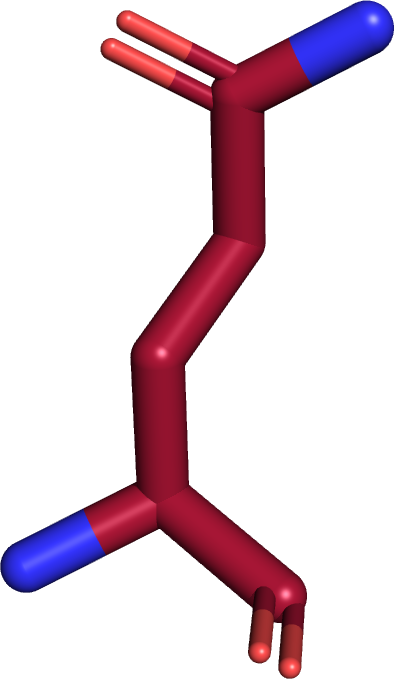
\includegraphics[width=0.25\columnwidth]{bioinfo/figures/amino_acid_Q}};
    \begin{scope}[x={(image.south east)},y={(image.north west)}]
    	\draw[Maroon, thick] (-0.05, -0.05) rectangle (0.85,0.3);
    	\draw[RoyalBlue, thick, dashed] (0.2, 0.35) rectangle (1.05, 1.05);
        %\draw[help lines,xstep=.1,ystep=.1] (0,0) grid (1,1);
        %\foreach \x in {0,1,...,9} { \node [anchor=north] at (\x/10,0) {0.\x}; }
        %\foreach \y in {0,1,...,9} { \node [anchor=east] at (0,\y/10) {0.\y}; }
    \end{scope}
\end{tikzpicture}
} %
\hfil %
\subcaptionbox{Tyrosine (Y) \label{subfig:aminoY}}{\begin{tikzpicture}
    \node[anchor=south west,inner sep=0] (image) at (0,0) {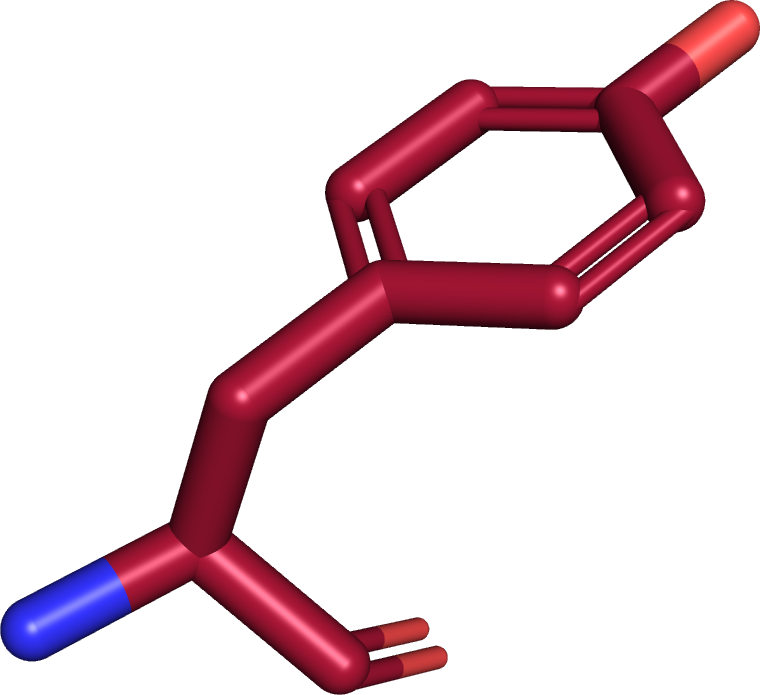
\includegraphics[width=0.45\columnwidth]{bioinfo/figures/amino_acid_Y}};
    \begin{scope}[x={(image.south east)},y={(image.north west)}]
	    \draw[Maroon, thick] (-0.05, -0.05) rectangle (0.6,0.3);
 	    \draw[RoyalBlue, thick, dashed] (0.2, 0.35) rectangle (1.05, 1.05);
        %\draw[help lines,xstep=.1,ystep=.1] (0,0) grid (1,1);
        %\foreach \x in {0,1,...,9} { \node [anchor=north] at (\x/10,0) {0.\x}; }
        %\foreach \y in {0,1,...,9} { \node [anchor=east] at (0,\y/10) {0.\y}; }
    \end{scope}
\end{tikzpicture}
} %
\hfil %
\caption{Two amino acids.
The maroon, solid rectangle indicates the backbone, common to all amino acids; and the blue dashed the side chain, that determines the specific chemical properties.}\label{fig:amino_acids}
\end{figure}



\subsection{Primary structure}
The amino acids can connect to each other through the peptide bond forming a chain.
The \emph{primary structure} is the sequence of amino acids as encoded in the DNA:
\begin{center}
\texttt{ALA ARG ILE ASN GLY ARG GLU ILE ASN VAL THR LYS LYS}
\end{center}

\subsection{Secondary structure}
%blabla hydrogen bonds
\ref{subfig:alpha}
\begin{figure}[hb]
	\centering
	\subcaptionbox{$\alpha$-helix\label{subfig:alpha}}{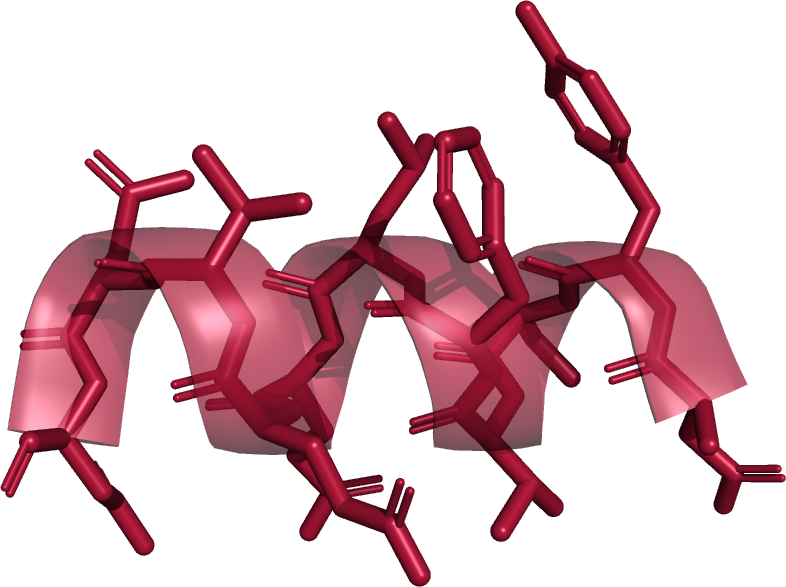
\includegraphics[width=0.9\textwidth]{bioinfo/figures/helix}}\\
	\subcaptionbox{$\beta$-sheet\label{subfig:beta}}{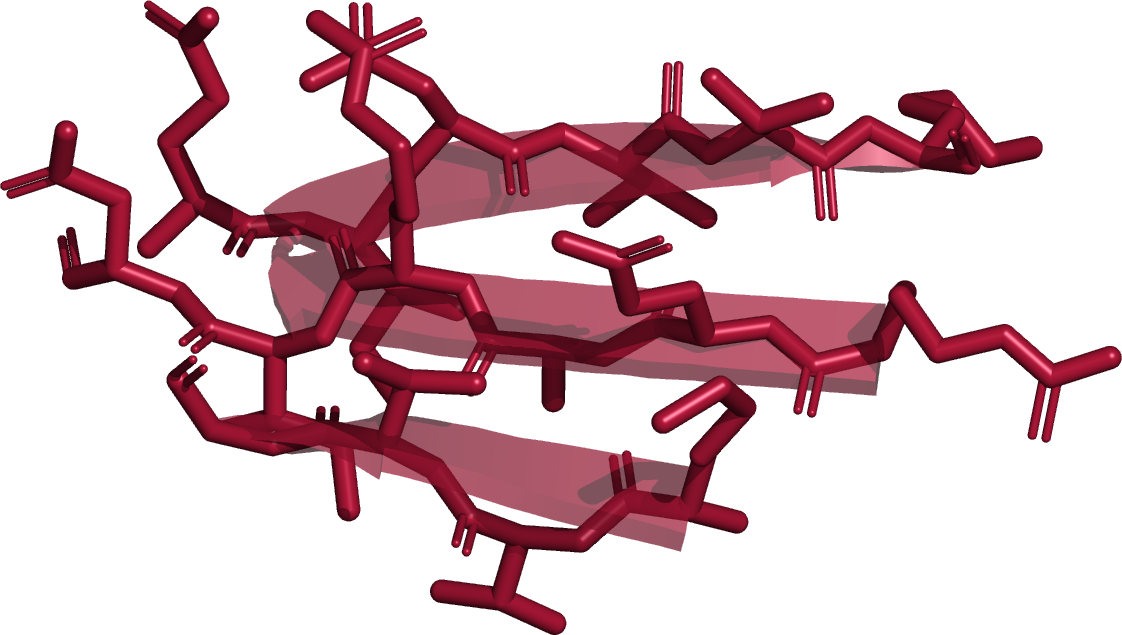
\includegraphics[width=0.9\textwidth]{bioinfo/figures/beta}}
	\caption{The two most frequent secondary structure elements.}\label{fig:alpha_beta}
\end{figure}


\subsection{Tertiary structure}
The spatial arrangement of the amino acids is called the \emph{tertiary structure},

\begin{figure}[htb]
\centering
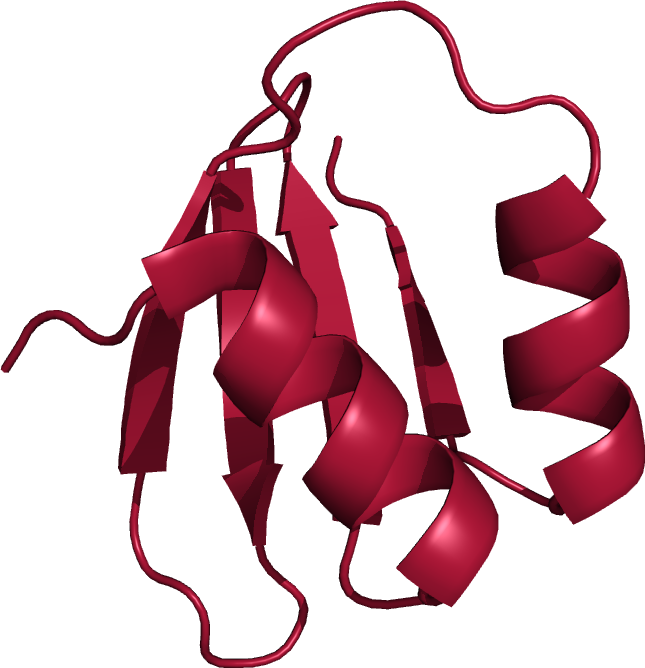
\includegraphics[width=0.9\textwidth]{bioinfo/figures/tertiary}
\caption{Tertiary structure of the chain B of the protein \texttt{4V0B}.}\label{fig:tertiary}
\end{figure}

\subsection{Quaternary structure}

\begin{figure}[htb]
\centering
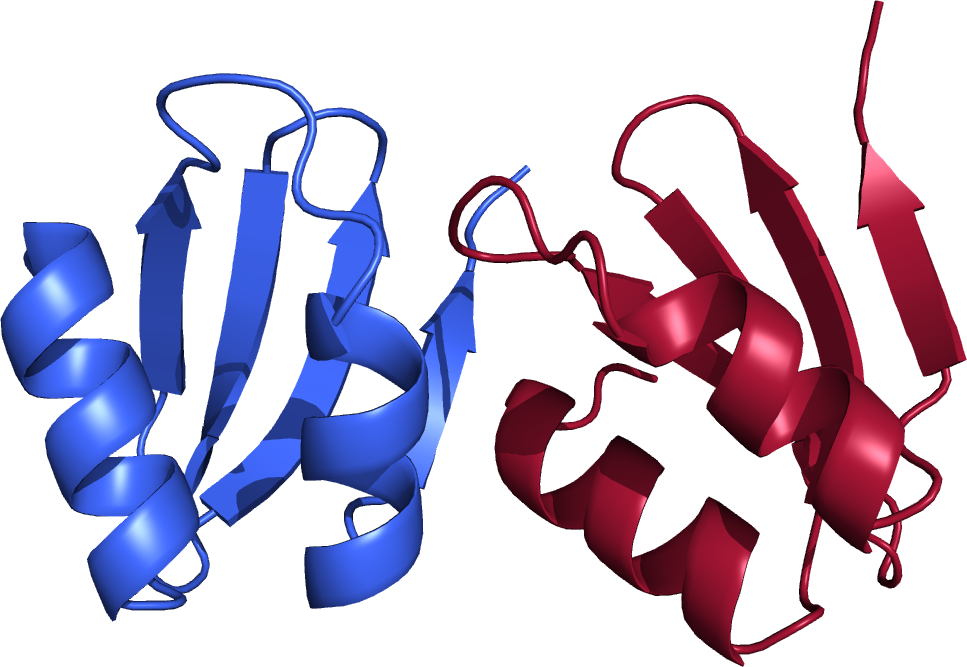
\includegraphics[width=0.9\textwidth]{bioinfo/figures/quaternary}
\caption{Quaternary structure of the chains A and B of the protein \texttt{4V0B}.}\label{fig:quaternary}
\end{figure}

\subsection{Quintenary structure} %?

\section{Protein biochemistry}
\subsection{Levinthal's paradox}
%cite how to fold graciously
\subsection{The protein backbone}
\subsection{Energy terms} %Force field
\subsection{The hydrophobic effect}

\section{Membrane proteins}
